\documentclass[conference,compsoc]{IEEEtran}
\ifCLASSOPTIONcompsoc
  \usepackage[nocompress]{cite}
\else
  \usepackage{cite}
\fi
\ifCLASSINFOpdf
\else
\fi

\usepackage{listings}

\usepackage{graphicx}
\graphicspath{ {images/} }

\begin{document}
\title{MemSan: Progress report}

\author{\IEEEauthorblockN{Hugo Genesse}
\IEEEauthorblockA{Computer Engineering\\
Polytechnique Montreal\\
Montreal, Quebec\\
hugo.genesse@polymtl.ca}}

\maketitle
\begin{abstract}
MemSan is a user-supplied data flow analyzer targeting memory-sensitize functions like strcpy that could lead to buffer overflow vulnerabilities.
\end{abstract}

\IEEEpeerreviewmaketitle



\section{Introduction}
% no \IEEEPARstart

The third part of the project was to construct the control flow graphs from the source code. We only had to create intra-procedural CFGs. The do and switch statements are still missing from the control flow graph for the moment.

\section{Methodology}

Clang's ASTRecursiveVisitor was still used for the part
 that builds our own AST. Some parts were added like: VisitBreakStmt,
 VisitContinueStmt, VisitUnaryOperator, TraverseForStmt, TraverseReturnStmt.
 Python classes for the analysis part of the project
 were once again added to ease the analysis.
 The code is available on github at svieg/MemSan.

\subsection{Implementation}

 For the C++ part, the logic didn't change apart from the additions discussed
 previously.

 Introduced in the second part of the project, Nodes were still used
 to interpret the output of the C++ part of the project. Although the core concept
 was the same (using nodes), a lot of refactoring had to take place to be able to walk
 the AST recursively as it eased the construction of the control flow graph. First,
 every node class was stripped down to only its name and then I added a node type to
 facilitate the implementation as I didn't need to check if the object was an instance
 of any node that could be possible. Every node was then added a children attribute
 that is a list of all its children. An edge will then be added between a parent node
 and a child node in the dumping process. The walk of the AST is split into two catefories:
 one is responsible for the dispatch to the right parse function according to the XML tag
 that it reads so we don't have to repeat the dispatch code in every parse function of every
 node type. The second one are the parser functions which every node type has one of. Every
 node type has its own steps required like the WhileNode which needs a whileEnd and whileBegin
 as well as a testing condition to break out of the loop. Similar logic has been implement for
 the ForNode as well as the ifNode. The others are simpler and only need to be linked to its
 immediate predecessor as it is the case for the unaryOperator, ContinueStmt and BreakStmt. The
 ReturnStmt is a special case has it need to linked to the exit node. The exit node is a singleton
 node that is the first to be created to be able to link to it without errors when GraphViz parses
 the output of our tool.

\section{Results and Discussion}

Sadly, I still couldn't get a real project to work on since I lacked time and had to work on a fake example provided in the lab.

\subsection{Results}

The CFG produced is included in the appendix. Some bugs are still present as you can see from the
figure. Firstly, the unaryOperator is in the wrong order as the returnStmt is currently a traverse
and the unaryOperator is treated like its child but it is the returnStmt that is linked to the
exit node. Secondly, some edges are missing and I couldn't find the bug in the logic in time.
 Thridly, some edges are duplicated as we can see in one of the return nodes. This is caused by the
 fact that the return node has multiple parents and causes the node to be visited multiple times and
 then the logic that is responsible for linking the return node to the exit nodes is executed
 multiple times.

\subsection{Difficulties}

\subsubsection{Compilation}

I didn't have time to spend on fixing the compilation for the chromium-os project.

\section{Conclusion}

I was able to create a CFG from C++ source code but only in
 the example I was provided and minor bugs.



% use section* for acknowledgment
\ifCLASSOPTIONcompsoc
  % The Computer Society usually uses the plural form
  \section*{Acknowledgments}
    Nicolas Cloutier, best teaching assistant.
\else
  % regular IEEE prefers the singular form
  \section*{Acknowledgment}
\fi

\section{Appendix}

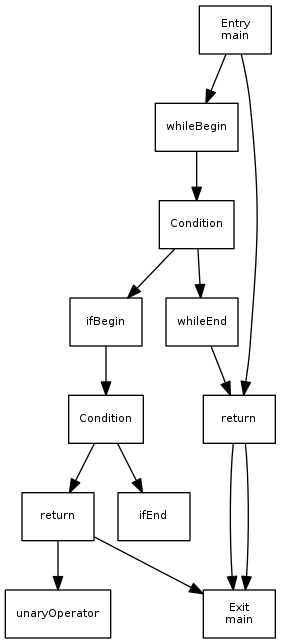
\includegraphics{cfg}

\end{document}


